\tikzstyle{neuron}=[circle,draw=blue!50,fill=blue!20,thick,minimum size=10mm]
\tikzstyle{input}=[circle,draw=black!50,fill=black!20,thick,minimum size=6mm]
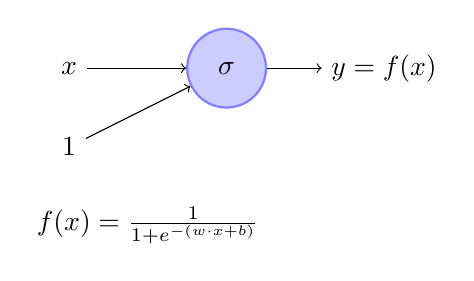
\begin{tikzpicture}
\node [neuron] (neuron0) at (1,6)  {$\sigma$} ;
\node (input1) at (-1,6)  {$x$};
\node (input0) at (-1,5)  {$1$};
\node (output0) at (3,6)  {$y = f(x)$};
\node (formula) at (0,4) {$f(x)= \frac{1}{1+e^{-(w\cdot x + b)}}$};
\draw [->] (input0) -- (neuron0);
\draw [->] (input1) -- (neuron0);
\draw [->] (neuron0) -- (output0);
\end{tikzpicture}
